\documentclass{article}
\usepackage{graphicx} % Required for inserting images

\title{Lista 2 - Modelagem Matemática}
\author{João Victor Barboza Machado das Neves}
\date{} % Deixe vazio para remover a data do \maketitle

\usepackage{amsmath}
\usepackage{graphicx}
\usepackage{float}
\usepackage{tikz}
\begin{document}

\maketitle

\section*{Exercício 1: Três Formulações para um Sistema}

Consideramos uma massa $m$ presa a uma mola de constante $k$, deslizando sobre uma superfície horizontal com coeficiente de atrito cinético $\mu$. A equação de movimento a ser obtida é
\[ m\ddot{u} + \mu m g\, \operatorname{sign}(\dot{u}) + k u = 0, \quad u(0) = u_0, \quad \dot{u}(0) = v_0. \]

\subsection*{(a) Derivação via 2ª Lei de Newton}

Adotamos a coordenada $u(t)$ medida na horizontal a partir da posição de equilíbrio da mola. As forças que atuam sobre a massa são:
\begin{itemize}
    \item \textbf{Força da mola} (Hooke): $F_s = -ku$, restauradora (opõe-se ao deslocamento).
    \item \textbf{Força de atrito cinético}: opõe-se sempre à \textit{velocidade}, com módulo $\mu N$ e sentido $-\operatorname{sign}(\dot{u})$, isto é, $F_{at} = -\mu N \operatorname{sign}(\dot{u})$.
    \item \textbf{Força normal} $N$ (vertical, para cima) e \textbf{peso} $mg$ (vertical, para baixo).
\end{itemize}

\begin{figure}[H]
    \centering
    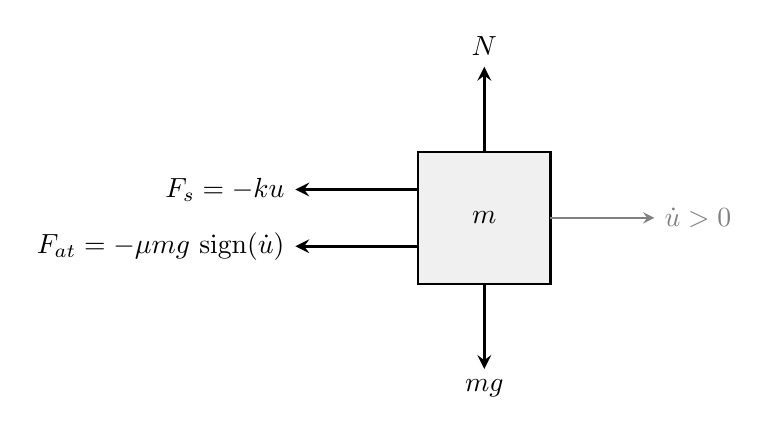
\begin{tikzpicture}[>=stealth, scale=1.2]
        \draw[thick, fill=gray!12] (-0.7,-0.7) rectangle (0.7,0.7);
        \node at (0,0) {$m$};
        \draw[->, very thick] (0,0.7) -- (0,1.6) node[above] {$N$};
        \draw[->, very thick] (0,-0.7) -- (0,-1.6) node[below] {$mg$};
        \draw[->, very thick] (-0.7,0.3) -- (-2.0,0.3) node[left] {$F_s = -ku$};
        \draw[->, very thick] (-0.7,-0.3) -- (-2.0,-0.3) node[left] {$F_{at} = -\mu m g\,\operatorname{sign}(\dot{u})$};
        \draw[->, thick, gray] (0.7,0) -- (1.8,0) node[right] {$\dot{u}>0$};
    \end{tikzpicture}
    \caption{Diagrama de corpo livre da massa (configuração ilustrada: $u>0$ e $\dot{u}>0$, com mola e atrito apontando no sentido negativo).}
\end{figure}

Na direção \textbf{vertical} não há movimento, logo o equilíbrio de forças fornece
\[ N - mg = 0 \implies N = mg, \]
de modo que o módulo do atrito é $\mu N = \mu m g$. Aplicando a 2ª lei de Newton na direção \textbf{horizontal},
\[ m\ddot{u} = \sum F_i = F_s + F_{at} = -ku - \mu m g\, \operatorname{sign}(\dot{u}). \]
Reorganizando, recuperamos a equação de movimento:
\[ m\ddot{u} + \mu m g\, \operatorname{sign}(\dot{u}) + k u = 0, \quad u(0) = u_0, \quad \dot{u}(0) = v_0. \]
O termo $\operatorname{sign}(\dot{u})$ é essencial: ele garante que o atrito troque de sentido sempre que a massa inverte o movimento, opondo-se sempre à velocidade.

\subsection*{(b) Formulação Lagrangiana (caso $\mu = 0$)}

Sem atrito o sistema é conservativo. Com a coordenada generalizada $q = u$:
\[ T = \tfrac{1}{2} m \dot{u}^2, \qquad V = \tfrac{1}{2} k u^2, \qquad L = T - V = \tfrac{1}{2} m \dot{u}^2 - \tfrac{1}{2} k u^2. \]
Calculando os termos da equação de Euler--Lagrange:
\[ \frac{\partial L}{\partial \dot{u}} = m\dot{u}, \qquad \frac{d}{dt}\!\left( \frac{\partial L}{\partial \dot{u}} \right) = m\ddot{u}, \qquad \frac{\partial L}{\partial u} = -ku. \]
Substituindo em $\dfrac{d}{dt}\!\left( \dfrac{\partial L}{\partial \dot{u}} \right) - \dfrac{\partial L}{\partial u} = 0$:
\[ m\ddot{u} - (-ku) = 0 \implies m\ddot{u} + k u = 0, \]
que é exatamente a equação de movimento sem atrito, confirmando a consistência com a formulação Newtoniana.

\subsection*{(c) Formulação Hamiltoniana (via transformada de Legendre)}

Tomamos o caso conservativo $\mu = 0$, coerente com o item (b), de modo que
$L = \tfrac{1}{2}m\dot u^2 - \tfrac{1}{2}ku^2$. A transformada de Legendre troca a
velocidade $\dot u$ pelo momento $p = \partial L/\partial \dot u$, produzindo uma
descrição em $(u,p)$ com o mesmo conteúdo físico de $L(u,\dot u)$. A troca é bem
definida porque $L$ é estritamente convexa em $\dot u$:
\[
\frac{\partial^2 L}{\partial \dot u^2} = m > 0,
\]
o que garante que $p = m\dot u$ é inversível.

\textbf{Momento e inversão.}
\[
p = \frac{\partial L}{\partial \dot u} = m\dot u
\qquad\Longrightarrow\qquad
\dot u = \frac{p}{m}.
\]

\textbf{Hamiltoniana.} Com $H = p\dot u - L$ e $\dot u$ escrito em função de $(u,p)$:
\[
H = p\cdot\frac{p}{m} - \left[\frac{1}{2}m\left(\frac{p}{m}\right)^2 - \frac{1}{2}ku^2\right]
= \frac{p^2}{2m} + \frac{1}{2}ku^2.
\]
Note que $H = T + V$. Isto não é definição, e sim consequência: vale porque $T$ é
quadrática em $\dot u$ e $V$ não depende de $\dot u$.

\textbf{Equações de Hamilton.}
\[
\dot u = \frac{\partial H}{\partial p} = \frac{p}{m},
\qquad
\dot p = -\frac{\partial H}{\partial u} = -ku.
\]
A primeira recupera a definição de momento; a segunda é a segunda lei de Newton
com a força restauradora da mola.

\textbf{Recuperando a equação de movimento.} Derivando a primeira equação e
substituindo a segunda:
\[
\ddot u = \frac{\dot p}{m} = -\frac{k}{m}\,u
\qquad\Longrightarrow\qquad
m\ddot u + ku = 0,
\]
idêntica à obtida em (a) e (b). Uma equação de segunda ordem foi substituída por
duas de primeira ordem, sem alterar a dinâmica.

\textbf{Conservação de $H$.} A estrutura antissimétrica das equações canônicas
força a conservação de $H$ ao longo de qualquer solução, independentemente da
forma específica do potencial:
\[
\frac{dH}{dt}
= \frac{\partial H}{\partial u}\dot u + \frac{\partial H}{\partial p}\dot p
= \frac{\partial H}{\partial u}\frac{\partial H}{\partial p}
+ \frac{\partial H}{\partial p}\left(-\frac{\partial H}{\partial u}\right) = 0.
\]

\textbf{Retrato de fase.} A condição $H = E$ constante,
\[
\frac{p^2}{2m} + \frac{1}{2}ku^2 = E,
\]
é a equação de uma família de elipses no plano $(u,p)$ — uma por nível de energia
$E$. As órbitas são fechadas (movimento periódico), percorridas no sentido
horário, e a origem é um centro estável. O retrato de fase exibe todas as
soluções simultaneamente, o que é a vantagem estrutural da formulação
Hamiltoniana sobre uma única trajetória.

\subsection*{(d) Por que o método lagrangiano padrão não trata o atrito}

O formalismo lagrangiano padrão ($L = T - V$) obtém as forças a partir de um \textbf{potencial escalar}: uma força admissível deve ser da forma $F = -\partial V/\partial q$, ou seja, derivável de uma função $V$ que dependa \textit{apenas das coordenadas}. O atrito $-\mu m g\, \operatorname{sign}(\dot{u})$ viola isso por três motivos:
\begin{enumerate}
    \item \textbf{Depende da velocidade}, não da posição: não existe $V(u)$ cujo gradiente $-\partial V/\partial u$ reproduza um termo em $\dot{u}$.
    \item \textbf{É dissipativo (não-conservativo)}: remove energia mecânica do sistema ao longo do movimento, e forças que dissipam energia não admitem potencial associado.
    \item \textbf{É não-suave}: $\operatorname{sign}(\dot{u})$ é descontínua em $\dot{u} = 0$, incompatível com a estrutura diferenciável exigida por $V$.
\end{enumerate}
Em resumo, forças dissipativas dependentes da velocidade ficam fora de $L = T - V$. O tratamento correto exige estender o formalismo — por exemplo, introduzindo uma \textbf{força generalizada} no lado direito da equação de Euler--Lagrange,
\[ \frac{d}{dt}\!\left( \frac{\partial L}{\partial \dot{u}} \right) - \frac{\partial L}{\partial u} = Q, \qquad Q = -\mu m g\, \operatorname{sign}(\dot{u}), \]
ou, equivalentemente, uma função de dissipação de Rayleigh.

\section*{Exercício 2: Conta em um Arame Rotativo}

Uma conta de massa $m$ desliza sem atrito ao longo de um arame reto que gira no
plano horizontal com velocidade angular constante $\omega$ em torno de um pivô fixo
numa extremidade. Seja $r(t)$ a distância da conta ao pivô.

\subsection*{(a) Energias cinética e potencial}

Como o arame gira com $\omega$ constante, o ângulo azimutal é imposto: $\varphi = \omega t$.
A conta tem então um único grau de liberdade, a coordenada radial $r$. Em coordenadas
polares, a velocidade tem componente radial $\dot r$ e componente tangencial $r\dot\varphi = r\omega$,
ortogonais entre si:
\[
v^2 = \dot r^2 + r^2\omega^2.
\]
A energia cinética é
\[
T = \tfrac{1}{2}m\left(\dot r^2 + r^2\omega^2\right).
\]
O movimento ocorre num plano horizontal, então a gravidade é perpendicular ao
deslocamento e não realiza trabalho. Não há outras forças conservativas, logo
\[
V = 0.
\]

\subsection*{(b) Lagrangiana e equação de movimento}

Com $V = 0$,
\[
L = T - V = \tfrac{1}{2}m\left(\dot r^2 + r^2\omega^2\right).
\]
As derivadas para Euler--Lagrange são
\[
\frac{\partial L}{\partial \dot r} = m\dot r,
\qquad
\frac{d}{dt}\!\left(\frac{\partial L}{\partial \dot r}\right) = m\ddot r,
\qquad
\frac{\partial L}{\partial r} = m r\omega^2.
\]
Substituindo em $\dfrac{d}{dt}\!\left(\dfrac{\partial L}{\partial \dot r}\right) - \dfrac{\partial L}{\partial r} = 0$:
\[
m\ddot r - m r\omega^2 = 0
\qquad\Longrightarrow\qquad
\ddot r = \omega^2 r.
\]

O sinal é o ponto a observar: a equação é $\ddot r = +\omega^2 r$, e não $\ddot r = -\omega^2 r$.
O termo $+mr\omega^2$ é a força centrífuga, que age como uma ``mola de rigidez
negativa'' — empurra a conta para fora, com intensidade crescente à medida que ela
se afasta do eixo.

\subsection*{(c) Solução e interpretação física}

A equação $\ddot r - \omega^2 r = 0$ é linear de segunda ordem com coeficientes
constantes. A equação característica $\lambda^2 - \omega^2 = 0$ tem raízes reais
$\lambda = \pm\omega$, de modo que a solução geral é hiperbólica (não oscilatória):
\[
r(t) = r_0\cosh(\omega t) + \frac{v_0}{\omega}\sinh(\omega t).
\]

\textbf{Para dentro ou para fora?} Genericamente, a conta \textit{escapa para fora}:
o termo $\cosh(\omega t)$ cresce exponencialmente e domina. O equilíbrio $r = 0$ é
\textbf{instável} — qualquer deslocamento ou velocidade inicial é amplificado. A
única exceção é a condição inicial finamente ajustada $v_0 = -\omega r_0$ (conta
lançada para dentro na velocidade exata), que anula o termo crescente e produz
\[
r(t) = r_0\, e^{-\omega t},
\]
um decaimento assintótico para o pivô. Fora desse caso-limite, a conta é expelida.

Fisicamente: no referencial girante, a força centrífuga não tem oposição neste
problema (o plano é horizontal, sem gravidade competindo), então nada confina a
conta. Isto contrasta com uma conta num aro girante sob gravidade, onde o termo
gravitacional restaurador compete com o centrífugo e gera um equilíbrio estável
fora do eixo — aqui esse contrapeso não existe.

\subsection*{(d) Quantidades conservadas}

\textbf{Coordenada cíclica.} A única coordenada generalizada é $r$, pois $\varphi = \omega t$
é prescrito e não constitui grau de liberdade. Verificamos se $r$ é cíclica:
\[
\frac{\partial L}{\partial r} = m r\omega^2 \neq 0.
\]
Logo $r$ \textbf{não} é cíclica, e o momento generalizado $p_r = \partial L/\partial\dot r = m\dot r$
\textbf{não} se conserva. Não há coordenada cíclica no problema reduzido, portanto
nenhum momento generalizado conservado. (O momento angular $L_z = m r^2\omega$ também
não se conserva: o motor exerce torque sobre o arame para manter $\omega$ constante à
medida que $r$ varia.)

\textbf{A energia $H = T + V$ é conservada?} Não. E o motivo é o cerne do exercício.
Como $L$ não depende explicitamente do tempo ($\omega$ é constante, e $\varphi$ já foi
eliminado), a simetria de translação temporal garante que a \textbf{função energia}
(integral de Jacobi) se conserva:
\[
h = \dot r\,\frac{\partial L}{\partial \dot r} - L
= m\dot r^2 - \tfrac{1}{2}m\left(\dot r^2 + r^2\omega^2\right)
= \tfrac{1}{2}m\dot r^2 - \tfrac{1}{2}m r^2\omega^2.
\]
Verificação direta:
\[
\frac{dh}{dt} = m\dot r\ddot r - m r\dot r\omega^2 = m\dot r\left(\ddot r - \omega^2 r\right) = 0
\quad\text{pela equação de movimento.}
\]

Ocorre que $h$ \textbf{não} é a energia mecânica $T + V$. Com $V = 0$, teríamos
$T + V = \tfrac{1}{2}m\dot r^2 + \tfrac{1}{2}m r^2\omega^2$, que difere de $h$ pelo
\textbf{sinal} do termo $\omega^2$. De fato, $T$ não se conserva:
\[
\frac{dT}{dt} = m\dot r\ddot r + m r\dot r\omega^2 = m\dot r\left(\ddot r + \omega^2 r\right)
= 2m\omega^2 r\dot r \neq 0.
\]

\textbf{Por que $h \neq T + V$.} A igualdade $H = T + V$ só vale quando $T$ é uma
função homogênea de grau dois nas velocidades generalizadas. Aqui isso falha: o
vínculo $\varphi = \omega t$ depende explicitamente do tempo, e ao eliminá-lo a energia
cinética se separa em duas partes,
\[
T = \underbrace{\tfrac{1}{2}m\dot r^2}_{T_2\ (\text{grau 2 em }\dot r)}
+ \underbrace{\tfrac{1}{2}m r^2\omega^2}_{T_0\ (\text{grau 0 em }\dot r)}.
\]
A função energia geral é $h = T_2 - T_0 + V$, e o termo $T_0$ entra com sinal
negativo. Substituindo, recupera-se exatamente $h = \tfrac{1}{2}m\dot r^2 - \tfrac{1}{2}m r^2\omega^2$.

\textbf{Interpretação física.} Sem atrito, seria natural esperar conservação de
energia. Mas o motor mantém $\omega$ constante realizando trabalho sobre o sistema, e
por isso a energia mecânica $T$ não se conserva. O que se conserva é $h$, que é a
energia medida no referencial girante: a energia cinética radial $\tfrac{1}{2}m\dot r^2$
menos o potencial centrífugo efetivo $\tfrac{1}{2}m r^2\omega^2$. Não por acaso, esse
potencial é a origem da força centrífuga $+mr\omega^2$ da equação de movimento —
derivá-lo em relação a $r$ (com sinal trocado) devolve exatamente esse termo.






\section*{Exercício 3: Escalamento do Pêndulo}

\subsection*{(a) Escalamento do pêndulo simples}
A equação governante é $m\ell\ddot{\theta} + mg\sin\theta = 0$, ou seja
\[ \ddot{\theta} + \frac{g}{\ell}\sin\theta = 0, \quad \theta(0) = \theta_0, \quad \dot{\theta}(0) = 0. \]
Como $\theta$ já é adimensional (um ângulo), só precisamos escalar o tempo. Introduzindo $\bar{t} = t/t_c$, a regra da cadeia dá $\ddot{\theta} = \frac{1}{t_c^2}\frac{d^2\theta}{d\bar{t}^2}$. Substituindo:
\[ \frac{1}{t_c^2}\frac{d^2\theta}{d\bar{t}^2} + \frac{g}{\ell}\sin\theta = 0 \implies \frac{d^2\theta}{d\bar{t}^2} + \frac{t_c^2 g}{\ell}\sin\theta = 0. \]
Escolhendo $t_c$ para tornar unitário o coeficiente do termo restaurador:
\[ \frac{t_c^2 g}{\ell} = 1 \implies t_c = \sqrt{\frac{\ell}{g}}. \]
A EDO escalada fica livre de parâmetros na equação:
\[ \frac{d^2\theta}{d\bar{t}^2} + \sin\theta = 0, \quad \theta(0) = \theta_0, \quad \frac{d\theta}{d\bar{t}}(0) = 0. \]
Permanece \textbf{um único parâmetro adimensional}, a amplitude inicial $\theta_0$, escondido na condição inicial.

\subsection*{(b) Pêndulo físico}
Para o pêndulo físico $I\ddot{\theta} + mg\ell\sin\theta = 0$, isto é $\ddot{\theta} + \frac{mg\ell}{I}\sin\theta = 0$, aplicamos o mesmo escalamento $\bar{t} = t/t_c$:
\[ \frac{d^2\theta}{d\bar{t}^2} + \frac{t_c^2\, mg\ell}{I}\sin\theta = 0. \]
Impondo coeficiente unitário:
\[ \frac{t_c^2\, mg\ell}{I} = 1 \implies t_c = \sqrt{\frac{I}{mg\ell}}. \]
A equação escalada é novamente $\dfrac{d^2\theta}{d\bar{t}^2} + \sin\theta = 0$, idêntica à do item (a).

\textbf{Comparação das escalas de tempo.} Temos $t_c = \sqrt{\ell/g}$ (simples) contra $t_c = \sqrt{I/(mg\ell)}$ (físico). Na forma escalada os dois problemas são \textit{sempre} a mesma equação: o escalamento absorve toda a informação dimensional dentro de $t_c$. Os dois pêndulos coincidem como sistemas \textbf{físicos} (mesma escala de tempo, logo mesmo período) exatamente quando as escalas se igualam:
\[ \sqrt{\frac{I}{mg\ell}} = \sqrt{\frac{\ell}{g}} \implies I = m\ell^2. \]
Isto é, quando o momento de inércia é o de uma massa pontual à distância $\ell$ do pivô --- o pêndulo simples é o caso particular $I = m\ell^2$ do pêndulo físico.

\subsection*{(c) Ângulo normalizado $\bar{\theta} = \theta/\theta_0$}
Para restringir a variável dependente ao intervalo $[0,1]$, definimos $\bar{\theta} = \theta/\theta_0$, ou seja $\theta = \theta_0\bar{\theta}$. Substituindo na equação escalada de (a):
\[ \theta_0\frac{d^2\bar{\theta}}{d\bar{t}^2} + \sin(\theta_0\bar{\theta}) = 0 \implies \frac{d^2\bar{\theta}}{d\bar{t}^2} + \frac{\sin(\theta_0\bar{\theta})}{\theta_0} = 0, \]
com $\bar{\theta}(0) = 1$ e $\bar{\theta}'(0) = 0$. Agora o parâmetro adimensional $\theta_0$ aparece \textbf{explicitamente} na equação, deixando de estar escondido na condição inicial.

\subsection*{(d) Faixa de validade da aproximação de pequenos ângulos}
Pela expansão de Taylor $\sin\theta = \theta - \frac{\theta^3}{6} + \cdots$, o erro absoluto ao aproximar $\sin\theta \approx \theta$ é $\theta - \sin\theta \approx \frac{\theta^3}{6}$. O erro relativo é, em ordem dominante,
\[ \frac{\theta - \sin\theta}{\theta} \approx \frac{\theta^3/6}{\theta} = \frac{\theta^2}{6}. \]
Exigindo precisão dentro de 5\%:
\[ \frac{\theta^2}{6} \le 0,05 \implies \theta^2 \le 0,3 \implies \theta \le \sqrt{0,3} \approx 0,548 \text{ rad}. \]
Convertendo para graus, $0,548 \times \frac{180}{\pi} \approx 31^\circ$. Portanto, a aproximação $\sin\theta \approx \theta$ é precisa dentro de 5\% para $|\theta_0| \lesssim 31^\circ$. \textit{Verificação exata:} em $\theta = 0,548$ rad, $\sin\theta \approx 0,521$, com erro relativo $\approx 5\%$, confirmando a estimativa de Taylor.

\section*{Exercício 4: Teorema de Noether — Conservação de $H$}

\subsection*{(a) Prova por cálculo direto}

Para uma Lagrangiana $L(q,\dot q)$ definimos a função energia
\[
H = \dot q\,\frac{\partial L}{\partial \dot q} - L.
\]
Vamos calcular $dH/dt$ no caso geral, sem supor de início que $L$ independe do
tempo, e só então especializar. Derivando pela regra do produto:
\[
\frac{dH}{dt}
= \ddot q\,\frac{\partial L}{\partial \dot q}
+ \dot q\,\frac{d}{dt}\!\left(\frac{\partial L}{\partial \dot q}\right)
- \frac{dL}{dt}.
\]
Se admitirmos dependência explícita no tempo, $L = L(q,\dot q,t)$, a regra da cadeia dá
\[
\frac{dL}{dt}
= \frac{\partial L}{\partial q}\dot q
+ \frac{\partial L}{\partial \dot q}\ddot q
+ \frac{\partial L}{\partial t}.
\]
Substituindo, o termo $\ddot q\,\partial L/\partial\dot q$ cancela e resta
\[
\frac{dH}{dt}
= \dot q\left[\frac{d}{dt}\!\left(\frac{\partial L}{\partial \dot q}\right)
- \frac{\partial L}{\partial q}\right]
- \frac{\partial L}{\partial t}.
\]
O colchete é precisamente o lado esquerdo da equação de Euler--Lagrange, que se
anula ao longo de qualquer trajetória física. Logo, na trajetória,
\[
\boxed{\;\frac{dH}{dt} = -\frac{\partial L}{\partial t}\;}
\]
Este é o resultado geral: a taxa de variação da função energia é menos a derivada
explícita de $L$ no tempo. No caso em que $L$ não depende explicitamente do tempo,
$\partial L/\partial t = 0$, obtém-se
\[
\frac{dH}{dt} = 0,
\]
ou seja, $H$ é conservado. Esta é a versão de Noether para a simetria de translação
temporal: se transladar a origem do tempo não altera a física ($L$ sem $t$
explícito), então existe uma quantidade conservada, e essa quantidade é $H$.

\subsection*{(b) Pêndulo simples}

Para $L = \tfrac{1}{2}m\ell^2\dot\theta^2 + mg\ell\cos\theta$, o momento generalizado é
\[
\frac{\partial L}{\partial \dot\theta} = m\ell^2\dot\theta,
\]
e a função energia fica
\[
H = \dot\theta\,\bigl(m\ell^2\dot\theta\bigr) - L
= m\ell^2\dot\theta^2 - \tfrac{1}{2}m\ell^2\dot\theta^2 - mg\ell\cos\theta
= \tfrac{1}{2}m\ell^2\dot\theta^2 - mg\ell\cos\theta.
\]
Comparando com a energia mecânica: $T = \tfrac{1}{2}m\ell^2\dot\theta^2$ e, como
$L = T - V$, lê-se $V = -mg\ell\cos\theta$. Portanto
\[
H = T + V = \tfrac{1}{2}m\ell^2\dot\theta^2 - mg\ell\cos\theta,
\]
que coincide com a energia total. A igualdade $H = T + V$ vale aqui porque $T$ é
quadrática homogênea em $\dot\theta$ e $V$ não depende de $\dot\theta$ — as duas
condições sob as quais a função energia é a energia mecânica. Como $L$ não depende
explicitamente do tempo, o item (a) garante que essa energia é conservada.

\subsection*{(c) Pêndulo duplo}

A Lagrangiana do pêndulo duplo é acoplada e não-linear, mas os vínculos são hastes
rígidas de comprimento fixo e a gravidade é estática: nada nela depende
explicitamente do tempo, $\partial L/\partial t = 0$. Pelo resultado de (a),
concluímos imediatamente que $H$ é conservado, \textbf{sem} precisar calcular sua
forma explícita. Além disso, como $T$ é quadrática homogênea nas velocidades
angulares e $V$ depende apenas dos ângulos, $H = T + V$ é a energia mecânica total.

\textbf{Uso como diagnóstico numérico.} O pêndulo duplo é um sistema caótico: não
possui solução analítica fechada e é sensível às condições iniciais, de modo que
não se pode validar uma trajetória numérica comparando-a com uma solução exata.
A conservação de $H$ oferece um teste independente. Como sabemos que $H$ deve
permanecer exatamente constante na dinâmica verdadeira, monitorar $H(t)$ ao longo
da simulação transforma qualquer deriva observada em medida direta do erro
numérico. Integradores não-simpléticos (por exemplo, Euler explícito) tipicamente
fazem $H$ derivar de forma sistemática, enquanto integradores simpléticos mantêm
$H$ oscilando dentro de uma faixa limitada. É um invariante barato de calcular e
serve como termômetro da qualidade do esquema.

\subsection*{(d) Pivô oscilante}

Considere agora um pêndulo cujo ponto de suporte oscila verticalmente segundo
$y_0(t) = A\cos(\omega t)$. A Lagrangiana passa a conter $y_0(t)$ e suas derivadas,
de modo que depende explicitamente do tempo: $\partial L/\partial t \neq 0$. Pelo
resultado geral de (a),
\[
\frac{dH}{dt} = -\frac{\partial L}{\partial t} \neq 0,
\]
e portanto $H$ \textbf{não} é conservado.

\textbf{Interpretação física.} O suporte é movido por um agente externo que impõe a
oscilação, e esse agente realiza trabalho sobre o pêndulo — injetando e removendo
energia ao longo do ciclo. O sistema é aberto: troca energia com o mecanismo que
agita o pivô, e a energia do pêndulo isolado não tem razão para se conservar. Do
ponto de vista de Noether, a oscilação do suporte distingue instantes de tempo — a
física em um dado momento não é a mesma de um instante deslocado —, o que quebra a
simetria de translação temporal. Sem essa simetria, não há quantidade de energia
conservada associada a ela.

\section*{Exercício 5: Escalamento do Sistema de Lotka--Volterra}

O sistema de Lotka--Volterra para presas $H$ e predadores $L$ é
\[
H' = H(a - bL), \qquad L' = L(dH - c), \qquad H(0) = H_0,\ L(0) = L_0,
\]
com $a,b,c,d > 0$. (Aqui $H$ e $L$ designam as duas populações, conforme o
enunciado.)

\subsection*{(a) Ponto estacionário e escalamento}

O equilíbrio não trivial exige $H' = L' = 0$ com ambas as populações positivas.
De $a - bL = 0$ e $dH - c = 0$:
\[
H^* = \frac{c}{d}, \qquad L^* = \frac{a}{b}.
\]
Usando esses valores como escalas características, $H_c = H^*$ e $L_c = L^*$, e uma
escala de tempo $t_c = 1/a$, definimos as variáveis adimensionais
\[
u = \frac{H}{H^*} = \frac{d}{c}H, \qquad
v = \frac{L}{L^*} = \frac{b}{a}L, \qquad
\tau = a\,t.
\]
Substituindo na primeira equação, com $H = \tfrac{c}{d}u$ e $L = \tfrac{a}{b}v$:
\[
\frac{c}{d}\,a\,\frac{du}{d\tau}
= \frac{c}{d}u\left(a - b\cdot\tfrac{a}{b}v\right)
= \frac{c}{d}\,a\,u(1 - v)
\quad\Longrightarrow\quad
\frac{du}{d\tau} = u(1 - v).
\]
Analogamente, na segunda equação:
\[
\frac{a}{b}\,a\,\frac{dv}{d\tau}
= \frac{a}{b}v\left(d\cdot\tfrac{c}{d}u - c\right)
= \frac{a}{b}\,c\,v(u - 1)
\quad\Longrightarrow\quad
\frac{dv}{d\tau} = \alpha\,v(u - 1),
\qquad \alpha = \frac{c}{a}.
\]
O sistema escalado é
\[
\frac{du}{d\tau} = u(1 - v),
\qquad
\frac{dv}{d\tau} = \alpha\,v(u - 1),
\qquad
\alpha = \frac{c}{a}.
\]
Resta um único parâmetro adimensional $\alpha$, contra os seis originais
($a,b,c,d,H_0,L_0$). Fisicamente, $\alpha = c/a$ é a razão entre a taxa de morte
do predador e a taxa de crescimento da presa. Note que este $\alpha$ é local a este
modelo e não tem relação com o parâmetro de mesmo nome usado no escalamento da
equação logística.

\subsection*{(b) Jacobiana e autovalores}

Com $F(u,v) = u(1 - v)$ e $G(u,v) = \alpha v(u - 1)$, a Jacobiana geral é
\[
J(u,v) =
\begin{bmatrix}
\partial_u F & \partial_v F \\[2pt]
\partial_u G & \partial_v G
\end{bmatrix}
=
\begin{bmatrix}
1 - v & -u \\[2pt]
\alpha v & \alpha(u - 1)
\end{bmatrix}.
\]
Os equilíbrios do sistema escalado são $(0,0)$ (ambas extintas) e $(1,1)$
(coexistência). Avaliando:
\[
J(0,0) =
\begin{bmatrix}
1 & 0 \\
0 & -\alpha
\end{bmatrix}
\quad\Longrightarrow\quad
\lambda_1 = +1, \quad \lambda_2 = -\alpha,
\]
\[
J(1,1) =
\begin{bmatrix}
0 & -1 \\
\alpha & 0
\end{bmatrix}
\quad\Longrightarrow\quad
\lambda^2 + \alpha = 0
\quad\Longrightarrow\quad
\lambda = \pm i\sqrt{\alpha}.
\]

\subsection*{(c) Classificação dos equilíbrios}

\textbf{Equilíbrio $(0,0)$.} Os autovalores $\lambda_1 = +1$ e $\lambda_2 = -\alpha$
são reais e de sinais opostos, o que caracteriza um \textbf{ponto de sela}
(instável). A direção instável é o eixo $u$: uma população de presas próxima de
zero cresce exponencialmente (regime de Malthus, na ausência de predadores). A
direção estável é o eixo $v$: predadores isolados, sem presa, morrem.

\textbf{Equilíbrio $(1,1)$.} Os autovalores $\lambda = \pm i\sqrt{\alpha}$ são
\textbf{imaginários puros}, o que caracteriza um \textbf{centro} (linearmente
neutro). As órbitas linearizadas em torno de $(1,1)$ são curvas fechadas,
percorridas com período $T = 2\pi/\sqrt{\alpha}$. Autovalores imaginários puros
indicam que, na vizinhança do equilíbrio, as trajetórias não se aproximam nem se
afastam: giram em torno dele em laços fechados, correspondendo a oscilações
sustentadas das duas populações.

Uma ressalva importante: um centro é \textit{estruturalmente frágil}. Em geral,
os termos não lineares desprezados na linearização podem convertê-lo em uma
espiral (atrativa ou repulsiva), de modo que a conclusão ``órbitas fechadas'' da
análise linear não sobrevive necessariamente ao sistema completo. No caso do
Lotka--Volterra, excepcionalmente, ela sobrevive — e a razão é o item (d).

\subsection*{(d) Primeira integral e órbitas fechadas}

Afirmamos que
\[
G(u,v) = \alpha u + v - \ln\!\left(u^{\alpha} v\right)
= \alpha u + v - \alpha\ln u - \ln v
\]
é uma quantidade conservada ao longo das soluções do sistema escalado.
Calculamos $dG/dt$ pela regra da cadeia. As derivadas parciais são
\[
\frac{\partial G}{\partial u} = \alpha - \frac{\alpha}{u} = \frac{\alpha(u - 1)}{u},
\qquad
\frac{\partial G}{\partial v} = 1 - \frac{1}{v} = \frac{v - 1}{v}.
\]
Substituindo as EDOs $u' = u(1 - v)$ e $v' = \alpha v(u - 1)$:
\[
\frac{dG}{dt}
= \frac{\alpha(u - 1)}{u}\,u(1 - v)
+ \frac{v - 1}{v}\,\alpha v(u - 1)
= \alpha(u - 1)(1 - v) + \alpha(v - 1)(u - 1).
\]
Colocando $\alpha(u - 1)$ em evidência:
\[
\frac{dG}{dt}
= \alpha(u - 1)\bigl[(1 - v) + (v - 1)\bigr]
= \alpha(u - 1)\cdot 0 = 0.
\]
Logo $G$ é constante ao longo de cada trajetória: é uma \textbf{primeira integral}
do sistema.

\textbf{Consequência sobre a forma das trajetórias.} A função $G$ é limitada
inferiormente e tem um mínimo estrito em $(1,1)$; seus conjuntos de nível em torno
desse ponto são curvas fechadas. Como cada órbita do sistema está inteiramente
contida em um conjunto de nível de $G$ (pois $G$ não varia ao longo dela), segue
que \textbf{toda} órbita no primeiro quadrante é uma curva fechada — não apenas as
órbitas da aproximação linear. É este fato que promove o centro: a linearização
apenas sugeria órbitas fechadas em torno de $(1,1)$, e a existência da primeira
integral $G$ confirma que elas de fato se fecham no sistema não linear completo,
resolvendo a fragilidade estrutural apontada em (c). As populações oscilam
indefinidamente, cada condição inicial permanecendo em seu próprio laço fechado.

Vale registrar o paralelo com a formulação Hamiltoniana: a função conservada $G$
desempenha aqui exatamente o papel que a Hamiltoniana $H(q,p)$ desempenhou nos
sistemas mecânicos — uma quantidade invariante cujos conjuntos de nível são as
próprias órbitas do sistema, provando que elas são fechadas. O centro do
Lotka--Volterra é, nesse sentido, o análogo ecológico do centro do oscilador
harmônico.

\section*{Exercício 6: O Limiar SIR e a Imunidade de Rebanho}

\subsection*{(a) Trajetória no plano de fase}

Partimos do sistema SIR escalado
\[
\frac{d\bar S}{d\bar t} = -R_0\,\bar S\,\bar I,
\qquad
\frac{d\bar I}{d\bar t} = R_0\,\bar S\,\bar I - \bar I = \bar I\,(R_0\bar S - 1),
\]
com $\bar S(0)=1$, $\bar I(0)=\alpha$. Dividindo a segunda equação pela primeira, o fator $\bar I$ se cancela e o tempo desaparece:
\[
\frac{d\bar I}{d\bar S}
= \frac{\bar I\,(R_0\bar S - 1)}{-R_0\,\bar S\,\bar I}
= -1 + \frac{1}{R_0\bar S}.
\]
O lado direito depende apenas de $\bar S$, e a integração é imediata:
\[
\bar I(\bar S) = -\bar S + \frac{1}{R_0}\ln\bar S + C.
\]
A condição inicial $\bar I(\bar S=1)=\alpha$ fixa $C = 1+\alpha$ (pois $\ln 1 = 0$), levando à trajetória
\[
\boxed{\;\bar I(\bar S) = 1 + \alpha - \bar S + \frac{1}{R_0}\ln\bar S\;}.
\]

Reescrita como $\bar I + \bar S - \tfrac{1}{R_0}\ln\bar S = 1+\alpha = \text{const}$, ela é uma primeira integral do sistema: cada trajetória vive sobre uma curva de nível dessa quantidade, exatamente o papel estrutural que $G(u,v)$ desempenha no sistema de Lotka--Volterra. A diferença qualitativa é decisiva. Como $d\bar S/d\bar t = -R_0\bar S\bar I < 0$ enquanto houver infecciosos, $\bar S$ é estritamente decrescente e o estado percorre a curva num único sentido, de $(\bar S,\bar I)=(1,\alpha)$ rumo ao fim da epidemia. Não há órbitas fechadas: em vez da oscilação sustentada do Lotka--Volterra, o fluxo unidirecional $S\to I\to R$ produz um surto transiente que se extingue.

\subsection*{(b) O pico da epidemia}

O pico de $\bar I$ ocorre quando $d\bar I/d\bar t = 0$. Da forma fatorada $d\bar I/d\bar t = \bar I(R_0\bar S - 1)$, descartando a raiz $\bar I=0$ (início e fim do surto), resta
\[
R_0\bar S^* - 1 = 0 \quad\Longrightarrow\quad \boxed{\;\bar S^* = \frac{1}{R_0}\;}.
\]
O mesmo valor sai de impor $d\bar I/d\bar S=-1+\tfrac{1}{R_0\bar S}=0$ na trajetória de (a), já que $d\bar S/d\bar t\neq 0$ no pico. A fração ainda suscetível no pico é, portanto, $\bar S^* = 1/R_0$.

Este é precisamente o limiar de imunidade de rebanho: enquanto $\bar S > 1/R_0$ a taxa efetiva $R_0\bar S$ excede 1 e a infecção cresce; quando $\bar S$ cruza $1/R_0$ por baixo, a fração $1-1/R_0$ já removida basta para inverter a tendência e a epidemia atinge seu ápice. Substituindo $\bar S^*$ na trajetória, a altura do pico é
\[
\bar I_{\max} = 1 + \alpha - \frac{1}{R_0}\bigl(1 + \ln R_0\bigr).
\]

\subsection*{(c) A fração suscetível final}

A epidemia termina quando $\bar I\to 0$ novamente. Impondo $\bar I=0$ na trajetória de (a):
\[
0 = 1 + \alpha - \bar S_\infty + \frac{1}{R_0}\ln\bar S_\infty
\quad\Longrightarrow\quad
\boxed{\;\bar S_\infty - \frac{1}{R_0}\ln\bar S_\infty = 1 + \alpha\;}.
\]
A função $f(\bar S)=\bar S - \tfrac{1}{R_0}\ln\bar S - (1+\alpha)$ tem $f'(\bar S)=1-\tfrac{1}{R_0\bar S}$, que se anula em $\bar S=1/R_0$ --- um mínimo. Como $f(1/R_0)=-\bar I_{\max}<0$, $f(\bar S)\to+\infty$ quando $\bar S\to 0^+$ e $f(1)=-\alpha<0$, há exatamente uma raiz no intervalo $(0,\,1/R_0)$. A raiz física $\bar S_\infty$ fica, portanto, abaixo do valor $\bar S^*=1/R_0$ do pico.

\subsection*{(d) Solução numérica e discussão}

Resolvendo a equação transcendental de (c) por um método de raiz (bisseção ou \texttt{scipy.optimize.fsolve}), com o bracket $(0,\,1/R_0)$ e $\alpha=0{,}02$:
\[
\begin{array}{lccc}
 & \bar S_\infty & \bar S^*=1/R_0 & 1+\alpha-\bar S_\infty \\[2pt]
R_0 = 2 & 0{,}190 & 0{,}50 & 0{,}830 \\
R_0 = 5 & 0{,}0063 & 0{,}20 & 1{,}014
\end{array}
\]
Para $R_0=2$, cerca de $83\%$ da população é infectada ao longo do surto. Para $R_0=5$, a fração final infectada é $1{,}014$, praticamente todo o total escalado $1+\alpha=1{,}02$ --- isto é, cerca de $99\%$ do conjunto inicial de suscetíveis. O aumento de $R_0$ tem efeito acentuado: $\bar S_\infty$ cai de $0{,}190$ para $0{,}006$, exaurindo quase por completo o compartimento suscetível.

Um ponto merece destaque. Em ambos os casos $\bar S_\infty \ll 1/R_0$: o surto não cessa ao atingir o limiar de imunidade de rebanho. No pico ($\bar S=1/R_0$) ainda há uma massa considerável de infecciosos ($\bar I_{\max}\approx 0{,}17$ para $R_0=2$ e $\approx 0{,}50$ para $R_0=5$), de modo que $d\bar S/d\bar t = -R_0\bar S\bar I$ permanece negativo e o consumo de suscetíveis prossegue muito além de $\bar S^*$. A epidemia ultrapassa o limiar por inércia, e é esse \emph{overshoot} que faz a fração final infectada superar $1-1/R_0$. O limiar $1/R_0$ marca onde a incidência começa a cair, não onde a transmissão se encerra.

\section*{Exercício 7: A Estrada Acidentada — Pipeline Completo}

\subsection*{(a) Solver de diferenças centradas e verificação}

Discretizamos $m\,u'' + b\,u' + k\,u = F(t)$ substituindo $u''$ pela segunda diferença centrada $[D_tD_t u]^n = (u^{n+1}-2u^n+u^{n-1})/\Delta t^2$ e $u'$ pela primeira diferença centrada $(u^{n+1}-u^{n-1})/(2\Delta t)$. Isolando $u^{n+1}$:
\[
u^{n+1} = \frac{2m\,u^n + \left(\tfrac{b\Delta t}{2}-m\right)u^{n-1} + \Delta t^2\left(F^n - k\,u^n\right)}{m + \tfrac{b\Delta t}{2}}.
\]
A recorrência de três níveis exige um primeiro passo. De uma expansão de Taylor de $u^1$ combinada com a EDO em $t=0$ (ou seja, $u''(0)=(F^0-b v_0-k u_0)/m$):
\[
u^1 = u_0 + \Delta t\,v_0 + \frac{\Delta t^2}{2m}\left(-b\,v_0 - k\,u_0 + F^0\right).
\]
O esquema é explícito, de segunda ordem e estável para $\Delta t < 2/\omega$, com $\omega=\sqrt{k/m}$.

\textbf{Verificação.} Com $b=0$, $k=\omega^2$, $F\equiv 0$, $u(0)=1$ e $u'(0)=0$, a solução exata é $u(t)=\cos(\omega t)$. Para $\omega=2$ e $\Delta t=2{,}5\times10^{-3}$, o solver reproduz a solução com erro máximo $8{,}25\times10^{-6}$, compatível com a convergência $\mathcal{O}(\Delta t^2)$ esperada.

\subsection*{(b) Perfil da estrada e montagem do forçamento}

O forçamento vem de derivar duas vezes no tempo o vetor posição da massa. As constantes geométricas (raio da roda, comprimento de repouso da mola, meia altura do corpo) desaparecem, restando $\ddot{\mathbf r}\cdot\hat{\jmath} = u''(t) + h''(vt)\,v^2$. A 2ª lei de Newton na vertical, descartando $-mg$ (que apenas desloca o equilíbrio) e tomando $s(u)=ku$, dá
\[
m\,u'' + b\,u' + k\,u = \underbrace{-m\,h''(vt)\,v^2}_{F(t)}.
\]
O fator $v^2$ é consequência da regra da cadeia: a estrada é função do espaço, $h(x)$, e o veículo a amostra em $x=vt$, de modo que $\tfrac{d^2}{dt^2}h(vt)=h''(vt)\,v^2$. Ou seja, o veículo responde à \textit{curvatura} da pista, não à sua altura. A curvatura é calculada por diferença centrada, $h''_i \approx (h_{i-1}-2h_i+h_{i+1})/\Delta x^2$, e as malhas espacial e temporal ficam acopladas por $\Delta t = \Delta x/v$. Como a montagem de $F$ envolve dupla diferenciação de $h$ — operação que amplifica ruído na ordem de $1/\Delta x^2$ — o perfil precisa ser suave. Adotou-se um perfil analítico regular (dois acidentes gaussianos e uma depressão, com amplitude de poucos centímetros), sobre o qual todo o restante do pipeline se aplica sem qualquer alteração.

\subsection*{(c) Simulação com parâmetros padrão}

Com $m=60$~kg, $k=60$~N/m, $b=80$~Ns/m e $v=5$~m/s, tem-se $\omega=\sqrt{k/m}=1$~rad/s, período $T\approx 6{,}3$~s e razão de amortecimento $\zeta=b/(2m\omega)\approx 0{,}67$ — sistema sub-amortecido. A Figura~\ref{fig:bumpy_default} mostra os três painéis: perfil da estrada, forçamento e deslocamento vertical. As oscilações rápidas do forçamento são filtradas; o veículo responde predominantemente perto de sua frequência natural, com o deslocamento decaindo entre os acidentes da pista.

\begin{figure}[H]
\centering

\includegraphics[width=0.85\textwidth]{bumpy_road_default.pdf}
\caption{Estrada, forçamento e deslocamento vertical para os parâmetros padrão.}
\label{fig:bumpy_default}
\end{figure}

\subsection*{(d) Varredura de parâmetros}

\textbf{Velocidade.} O painel superior da Figura~\ref{fig:bumpy_sweep} mostra o deslocamento em função da distância para $v=5$, $10$ e $20$~m/s. A amplitude do forçamento cresce exatamente como $v^2$ (picos de $37{,}5$, $150$ e $600$~N — fatores de $4$ e $16$), mas o deslocamento \textit{satura}: os picos vão de $38$ para $49$ e $50$~mm. A razão é que a frequência com que os acidentes são atravessados cresce com $v$, empurrando o forçamento para o regime dominado pela inércia, onde a resposta escala como $F/\Omega^2$. Como $F\sim v^2$ e a frequência dominante $\Omega\sim v$, os dois efeitos quase se cancelam e o deslocamento torna-se praticamente independente de $v$ em alta velocidade: a suspensão atua como um filtro passa-baixa.

\textbf{Amortecimento.} Fixando $v=5$~m/s (painel inferior), $b=40$, $80$ e $200$~Ns/m correspondem a $\zeta=0{,}33$, $0{,}67$ e $1{,}67$. Quanto maior o amortecimento, menor a amplitude e menos oscilação residual: o pico de deslocamento cai de $55{,}6$ para $38{,}0$ e $22{,}1$~mm. O caso sub-amortecido ($\zeta=0{,}33$) oscila visivelmente entre os acidentes, ao passo que o super-amortecido ($\zeta=1{,}67$) responde de forma lenta e sem oscilação, com a menor amplitude.

\begin{figure}[H]
\centering

\includegraphics[width=0.85\textwidth]{bumpy_sweep.pdf}
\caption{Varredura em velocidade (superior) e em amortecimento (inferior).}
\label{fig:bumpy_sweep}
\end{figure}

\section*{Exercício 8: Modelo SIR — Explorando Dinâmicas Epidêmicas}

\subsection*{(a) Solver e lei de conservação}

O lado direito do sistema SIR escalado é implementado diretamente:
\[
\frac{d\bar S}{d\bar t}=-R_0\bar S\bar I,\qquad
\frac{d\bar I}{d\bar t}=R_0\bar S\bar I-\bar I,\qquad
\frac{d\bar R}{d\bar t}=\bar I,
\]
com $\bar S(0)=1$, $\bar I(0)=\alpha$, $\bar R(0)=0$, integrado por \texttt{solve\_ivp} (RK45, \texttt{rtol}$=10^{-9}$). Somando as três equações, $\frac{d}{d\bar t}(\bar S+\bar I+\bar R)=0$, de modo que $\bar S+\bar I+\bar R=1+\alpha$ em todo instante. Usada como diagnóstico numérico, essa lei é preservada com violação máxima de $6{,}66\times10^{-16}$ ao longo de toda a simulação — no nível do arredondamento de ponto flutuante, confirmando que o erro do integrador é desprezível.

\subsection*{(b) Curvas de referência para $R_0=2$ e $R_0=5$}

A Figura~\ref{fig:sir_ref} mostra $\bar S$, $\bar I$, $\bar R$ para os dois valores. Para $R_0=2$ o surto é moderado: $\bar I$ atinge o pico em $0{,}173$ e cerca de $83\%$ da população se recupera. Para $R_0=5$ o surto é severo: $\bar I$ chega a $0{,}498$ e praticamente toda a população é infectada. Os picos numéricos coincidem com os valores $\bar I_{\max}=1+\alpha-\tfrac{1}{R_0}(1+\ln R_0)$ obtidos analiticamente no Exercício~6, o que valida o solver contra a solução exata da trajetória.

\begin{figure}[H]
\centering

\includegraphics[width=0.9\textwidth]{sir_reference.pdf}
\caption{Dinâmica SIR escalada para $R_0=2$ (moderado) e $R_0=5$ (severo).}
\label{fig:sir_ref}
\end{figure}

\subsection*{(c) Varredura em $R_0$}

Varrendo $R_0$ de $0{,}5$ a $6$ (com $\alpha=0{,}01$), registram-se o pico de $\bar I$ e a fração final infectada $1+\alpha-\bar S_\infty$ (Figura~\ref{fig:sir_sweep}). O comportamento de limiar é nítido: para $R_0<1$ não há surto — o pico de $\bar I$ permanece no valor inicial $\alpha$ e a fração infectada é praticamente nula —, pois $\dot{\bar I}(0)=\alpha(R_0-1)<0$. A partir de $R_0=1$, ambas as grandezas crescem acentuadamente, e já por volta de $R_0\approx 4$ quase toda a população é infectada. A linha vertical tracejada marca o limiar $R_0=1$.

\begin{figure}[H]
\centering

\includegraphics[width=0.9\textwidth]{sir_r0_sweep.pdf}
\caption{Pico de $\bar I$ (esquerda) e tamanho final da epidemia (direita) em função de $R_0$. O surto só existe para $R_0>1$.}
\label{fig:sir_sweep}
\end{figure}

\subsection*{(d) Extensão SIRV}

Acrescentam-se dois mecanismos: perda de imunidade a uma taxa $\gamma$ (recuperados voltam a suscetíveis) e vacinação a uma taxa $\delta(\bar t)$ (suscetíveis migram para o compartimento $\bar V$):
\[
\begin{aligned}
\frac{d\bar S}{d\bar t}&=-R_0\bar S\bar I+\gamma\bar R-\delta\bar S, &
\frac{d\bar I}{d\bar t}&=R_0\bar S\bar I-\bar I,\\
\frac{d\bar R}{d\bar t}&=\bar I-\gamma\bar R, &
\frac{d\bar V}{d\bar t}&=\delta\bar S,
\end{aligned}
\]
com $\gamma=0{,}05$ e uma campanha $\delta=0{,}5$ ativa em $\bar t\in[7,15]$ (e $\delta=0$ fora dela). A soma das quatro equações continua nula, então $\bar S+\bar I+\bar R+\bar V=1+\alpha$ permanece conservado. A Figura~\ref{fig:sirv} compara os dois cenários com $R_0=5$. Sem vacinação, a perda de imunidade realimenta o compartimento suscetível e produz \textit{ondas recorrentes} que se estabilizam num regime endêmico, em vez de um único surto. A campanha desvia suscetíveis para $\bar V$ durante a janela, cortando a transmissão e suprimindo as ondas seguintes.

Como o modelo permite reinfecção, a carga total é medida pelo fluxo cumulativo de novas infecções, $\int_0^{\bar t_f} R_0\bar S\bar I\,d\bar t$. A campanha reduz esse total de $3{,}10$ para $1{,}95$ — uma queda de aproximadamente $37\%$.

\begin{figure}[H]
\centering

\includegraphics[width=0.9\textwidth]{sirv_comparison.pdf}
\caption{Dinâmica SIRV ($R_0=5$): sem vacinação (ondas recorrentes) versus campanha de vacinação em $\bar t\in[7,15]$ (faixa sombreada).}
\label{fig:sirv}
\end{figure}

\end{document}




